\documentclass[12pt,letterpaper]{article}

%% Packages
\usepackage[margin=1.0in]{geometry}
\usepackage{amsmath,amssymb}
\usepackage{graphicx}
\usepackage[numbers,sort&compress]{natbib}
\usepackage{hyperref}
\usepackage{booktabs}
\usepackage{microtype}
\usepackage{setspace}
\usepackage{xcolor}
\usepackage{caption}
\usepackage[utf8]{inputenc}
\usepackage[T1]{fontenc}
\usepackage{lmodern}
\usepackage{listings}
\usepackage{color}

\lstdefinestyle{pythonstyle}{
  language=Python,
  basicstyle=\footnotesize\ttfamily,
  keywordstyle=\color{blue!75!black}\bfseries,
  commentstyle=\color{green!45!black}\itshape,
  stringstyle=\color{red!55!black},
  numbers=left,
  numberstyle=\tiny\color{gray!70},
  stepnumber=5,
  numbersep=8pt,
  showstringspaces=false,
  breaklines=true,
  breakatwhitespace=false,
  frame=tb,
  framesep=4pt,
  xleftmargin=22pt,
  xrightmargin=4pt,
  tabsize=4,
  captionpos=b,
  literate={--}{{-{}-}}2,
}
\lstset{style=pythonstyle}


\singlespacing
\setlength{\parskip}{0.4em}
\setlength{\parindent}{1.5em}

\hypersetup{
  colorlinks=true,
  linkcolor=blue!60!black,
  citecolor=blue!60!black,
  urlcolor=blue!60!black
}

\bibliographystyle{unsrtnat}

\captionsetup{font=small, labelfont=bf}

%% Title
\title{\textbf{The White Dwarf Mass--Radius Relation:\\
A Numerical Study Using the Chandrasekhar Equation of State}}
\author{Bhaskar Jain, Anika Chawla, Ellen Wang, Amita Anand\\[4pt]
        \small PHYS 6260: Computational Astrophysics\\[2pt]
        \small Spring 2026}
\date{}

% ============================================================
\begin{document}
\maketitle
\thispagestyle{empty}

% ============================================================
\section{Introduction}
\label{sec:intro}

White dwarfs are the end state for roughly 97\% of all stars in the Galaxy,
incluing our own Sun for the Earth \citep{fontaine2001}.
When a low or intermediate mass star ($M \lesssim 8\,M_\odot$) runs out of nuclear fuel,
it sheds its outer layers as a planetary nebula, which is an interesting and cool process, and leaves behind a degenerate
carbon-oxygen core, typically containing $0.5$--$1.2\,M_\odot$ of material squeezed
into a volume roughly the size of Earth (quite dense).
With no nuclear burning capability left because of the lack of fuel, the whole thing is held up by the quantum mechanical
degeneracy pressure of the electron gas. This is a phenomenon first explained by Fowler
\citep{fowler1926}.

This entire deal was put in a a firm theoretical footing by Chandrasekhan,
who in 1931 showed that a cold degenerate star cannot exceed a certain maximum mass.
Nowe we call this the Chandrasekhar limit \citep{chandrasekhar1931}\citep{chandrasekhar1939}.
The key insight is that as the stellar mass grows, the electrons get more and more
relativistic, and in the fully relativistic limit the equation of state softens from
$\Gamma = 5/3$ toward $\Gamma = 4/3$, at which point hydrostatic equilibrium can no
longer be maintained.

We will be looking at tthe white dwarf mass-radius (M--R) relation, which is useful because it directly encodes the
equation of state in an observable form. It essentially gives us a relationship between the mass and radius of a white dwarf at fixed composition, the radius decreases
monotonically with mass (while it actually approaches zero at the Chandrasekhar limit).
Testing this against real stars is the purpose of this project. As a first reason, it checks whether
Chandrasekhar's framework holds (basically is this model valid and how valid is it), and any deviations from the zero-temperature curve
can point to physics we left out of our modelling efforts, like finite temperature, Coulomb corrections
\citep{salpeter1961,hamada1961}, element stratification, or general-relativistic
corrections to pressure balance \citep{shapiro1983}.

Observational tests of the M--R relation that we are testing and using here in this paper only became practical once high-quality
astrometry was available. This is naturally past the time of Chandrasekhar so he could not do this, so we will do it for him.
Something interesting is that \citet{provencal1998} used \textit{Hipparcos} parallaxes to measure radii for
nearby white dwarfs with masses from orbital dynamics or spectroscopy, which we will use for data later (Section \ref{sec:data}).

Section~\ref{sec:theory} derives the governing equations.
Section~\ref{sec:numerics} describes the integration method.
Section~\ref{sec:data} covers the dataset.
Section~\ref{sec:results} presents results and
Section~\ref{sec:conclusions} gives our conclusions.

% ============================================================
\section{Theoretical Framework}
\label{sec:theory}

\subsection{Stellar Structure Equations}

For our project, we begin with a spherically symmetric, non-rotating star in hydrostatic equilibrium for our problem. It obeys
two coupled ordinary differntial equations (ODEs) that we are concerned with.
The first is the pressure-gravity balance:
\begin{equation}
  \frac{dP}{dr} = -\frac{G\,M(r)\,\rho(r)}{r^2},
  \label{eq:hse}
\end{equation}
where $P(r)$ is the pressure, $\rho(r)$ is the mass density, $G$ is the gravitational
constant, and $M(r)$ is the enclosed mass at radius $r$.
The second equation is mass continuity:
\begin{equation}
  \frac{dM}{dr} = 4\pi r^2\,\rho(r).
  \label{eq:mass}
\end{equation}
Both hold from the center ($r = 0$) out to the stellar surface where $P(R) = 0$.
To close the system we need an equation of state $P = P(\rho)$.

\subsection{The Chandrasekhar Equation of State}
\label{sec:eos}

In a cold ($T = 0$) white dwarf, we can say that all of the pressure comes from the degenerate electron
gas. We will add some detail to this this so that electrons fill momentum space up to the Fermi momentun $p_F$, with all states below
occupied and all states above empty.
The electron number density relates to $p_F$ through the Fermi sphere volume,
including the spin factor of 2:
\begin{equation}
  n_e = \frac{p_F^3}{3\pi^2\hbar^3}.
  \label{eq:ne}
\end{equation}
In an extreme case. For a fully ionized plasma with mean molecular weight per electron $\mu_e$
(equal to 2 for carbon or oxygen), the mass density is $\rho = \mu_e m_H n_e$,
where $m_H$ is the proton mass.

The dimensionless Fermi momentum
\begin{equation}
  x \;\equiv\; \frac{p_F}{m_e c},
  \label{eq:xdef}
\end{equation}
with $m_e$ the electron mass and $c$ the speed of light.
In term of $x$ the desnity takes the form
\begin{equation}
  \rho = B\,x^3,
  \qquad
  B \;\equiv\; \frac{\mu_e\,m_H}{3\pi^2\,\lambda_e^3},
  \label{eq:rho_x}
\end{equation}
where $\lambda_e = \hbar/(m_e c) = 3.862 \times 10^{-11}$\,cm is the reduced electron
Compton wavelength.
Numerically $B = \dfrac{\mu_e m_H}{3\pi^2 \lambda_e^3} = 1.96 \times 10^6$\,g\,cm$^{-3}$ for $\mu_e = 2$.

The pressure of a relativistic degenerate electron gas comes from the kinetic-theory
formula
\begin{equation}
  P = \frac{1}{3}\cdot\frac{2}{h^3}\int_0^{p_F}
        v(p)\,p\cdot 4\pi p^2\,dp,
  \label{eq:Pintegral}
\end{equation}
where $v(p) = pc^2/\sqrt{p^2c^2 + m_e^2c^4}$ is the relativistic group velocity and
the factor of 2 acocunts for electron spinn.
Substituting $p = m_e c\,t$ and evaluating the integral analytically gives
\begin{equation}
  P = A\,f(x),
  \qquad
  A \;\equiv\; \frac{m_e c^2}{24\pi^2\lambda_e^3}
    = \frac{\pi m_e^4 c^5}{3h^3},
  \label{eq:P_x}
\end{equation}
where $h = 2\pi\hbar$ is Planck's constant and the Chandrasekhar function is
\begin{equation}
  f(x) = x\bigl(2x^2 - 3\bigr)\sqrt{1+x^2} + 3\sinh^{-1}(x).
  \label{eq:fx}
\end{equation}
Numerically $A = 6.00 \times 10^{22}$\,dyn\,cm$^{-2}$.
Together, equations~\eqref{eq:rho_x} and~\eqref{eq:P_x} give the EOS parametrically
through $x$.

We also need $dP/d\rho$ in closed fom.
Differentiating equations~\eqref{eq:rho_x} and~\eqref{eq:P_x} with respect to $x$:
\begin{align}
  \frac{dP}{dx}   &= A\,\frac{8x^4}{\sqrt{1+x^2}},
  \label{eq:dPdx}\\
  \frac{d\rho}{dx} &= 3B\,x^2,
  \label{eq:drhodx}
\end{align}
from which
\begin{equation}
  \frac{dP}{d\rho} = \frac{dP/dx}{d\rho/dx}
    = \frac{8A\,x^2}{3B\,\sqrt{1+x^2}}.
  \label{eq:dPdrho}
\end{equation}


\subsection{Limiting Cases and the Chandrasekhar Mass}

\paragraph{Non-relativistic limit ($x \ll 1$).}
Expanding $f(x)$ for smalll $x$ gives $f(x) \approx (8/5)x^5$, so
\begin{equation}
  P \approx K_\mathrm{NR}\,\rho^{5/3},
  \qquad
  K_\mathrm{NR} = \frac{8A}{5\,B^{5/3}}.
  \label{eq:PNR}
\end{equation}
This is an $n = 3/2$ polytrope ($\Gamma = 5/3$), which gives $R \propto M^{-1/3}$. From this
we can say that less massive wihte dwarfs are physically larger naturally making sense.

\paragraph{Ultrarelativistic limit ($x \gg 1$).}
For large $x$, $f(x) \approx 2x^4$, giving
\begin{equation}
  P \approx K_\mathrm{UR}\,\rho^{4/3},
  \qquad
  K_\mathrm{UR} = \frac{2A}{B^{4/3}}.
  \label{eq:PUR}
\end{equation}
This is an $n = 3$ polytrope ($\Gamma = 4/3$),

As $\rho_c \to \infty$ the stellar mass asymptotes to \citep{chandrasekhar1931,shapiro1983}:
\begin{equation}
  M_\mathrm{Ch} = \frac{5.87}{\mu_e^2}\,M_\odot
  \approx 1.47\,M_\odot \quad (\mu_e = 2).
  \label{eq:Mch}
\end{equation}
Above this limti, no amount of compression can restore hydrostatic balance. Thus so no
cold non-rotating white dwarf can ever exceed it.

% ============================================================
\section{Numerical Method}
\label{sec:numerics}

\subsection{Reformulation as an Initial Value Problem}

Equations~\eqref{eq:hse}--\eqref{eq:mass} are technically a two-point boudary value
problem: we know $M(0) = 0$ and $P(R) = 0$, but we don't know $R$ ahead of time.
The standard trick is to turn this into an initial value problem (IVP) by picking
a central density $\rho_c$ and just integrating outward \citep{prialnik2000}.
Using the state vector $\mathbf{y}(r) = [M(r),\;\rho(r)]$ and the chain rule:
\begin{equation}
  \frac{d}{dr}\begin{pmatrix}M\\\rho\end{pmatrix}
  =
  \begin{pmatrix}4\pi r^2\,\rho\\[4pt]
  -\dfrac{G\,M\,\rho}{r^2\,(dP/d\rho)}\end{pmatrix},
  \label{eq:ode_system}
\end{equation}
where $dP/d\rho$ is given by equation~\eqref{eq:dPdrho}.
Using $\rho$ instead of $P$ as the second state variable avoids having to invert
$P \mapsto \rho$ at every step, which is nice for our group.

\subsection{Initial Conditions}

To avoid the singularity at $r = 0$ we start the integration at $r_0 = 10^3$\,cm
(= 10\,m).
At that point we set
\begin{equation}
  M(r_0) = \tfrac{4}{3}\pi r_0^3\,\rho_c,
  \label{eq:ic}
\end{equation}
and $\rho(r_0) = \rho_c$.
No special matching near the origin is needed. 
Tis is because the mass enclosed at $r_0$ is completely negligble compared to the total stellar mass.

\subsection{Integration Scheme}

We integrate using \texttt{scipy.integrate.solve\_ivp}
\citep{dormand1980} \citep{virtanen2020}.
We set relative and absolute tolerances of $10^{-8}$ and $10^{-10}$, respecttively, and cap the
maximum step size at $5 \times 10^6$\,cm (50\,km) to avoid taking steps that are
too large near the surface, which might have intersting behaviors.

The integration stops when $P(\rho) \leq 10^{-6} P(\rho_c)$. 
The stellar radius $R$ and total mass $M_\star = M(R)$ are recorded at that point.

\subsection{Grid and Convergence}

We run this for 120 central densities log-spaced over
$\rho_c \in [10^4,\,10^{10}]\,\mathrm{g\,cm^{-3}}$.
The lower bound gives very low-mass white dwarfs ($M \lesssim 0.15\,M_\odot$,
$R \approx 0.02\,R_\odot$) while the upper bound ($x_c \approx 17$) gets us within
$\sim 0.01\,M_\odot$ of the Chandrasekhar limit.

% ============================================================
\section{Observational Data}
\label{sec:data}
The six white dwarfs in our comparison are listed in Table~\ref{tab:obs}.
The Provencal et al.\ sample spnas masses $0.50$--$0.79\,M_\odot$, covering the
bulk of the typical white dwarf mass range, while Sirius~B at $1.02\,M_\odot$
tests the high-mass end near the Chandrasekhar regime.

\begin{table}[htbp]
  \centering
  \caption{Observed white dwarf masses and radii used for comparison.
           All uncertainties are $1\sigma$.}
  \label{tab:obs}
  \begin{tabular}{lcccl}
    \toprule
    Star & $M\,(M_\odot)$ & $R\,(R_\odot)$ & $R$\,(km) & Reference \\
    \midrule
    Sirius B      & $1.018 \pm 0.011$ & $0.00864 \pm 0.00012$ & $6009 \pm 83$  & \citet{barstow2005}   \\
    40 Eri B      & $0.501 \pm 0.011$ & $0.01360 \pm 0.00020$ & $9454 \pm 139$ & \citet{provencal1998} \\
    Procyon B     & $0.604 \pm 0.018$ & $0.00960 \pm 0.00050$ & $6676 \pm 348$ & \citet{provencal1998} \\
    Stein 2051 B  & $0.500 \pm 0.050$ & $0.01110 \pm 0.00070$ & $7717 \pm 487$ & \citet{provencal1998} \\
    EG 50         & $0.550 \pm 0.030$ & $0.01240 \pm 0.00100$ & $8622 \pm 695$ & \citet{provencal1998} \\
    GD 140        & $0.790 \pm 0.030$ & $0.00850 \pm 0.00100$ & $5909 \pm 695$ & \citet{provencal1998} \\
    \bottomrule
  \end{tabular}
\end{table}

% ============================================================
\section{Results and Discussion}
\label{sec:results}

\subsection{The Mass--Radius Curve}

Figure~\ref{fig:mr} shows the computed M--R curve with the observational data overlaid.
Starting from large radii at low masses,
the radius decreases monotonically with mass, assymptotically approaching zero as we
get close to the Chandrasekhar limit (Note: the vertical dashed line marks the numerically determined Chandrasekhar
mass limit).
The secondary $y$-axis on the right gives the radius in kilometres.
Observational data are from \citet{provencal1998} and \citet{barstow2005}, which you can see in Table~\ref{tab:obs}.
           

At low masses ($M \lesssim 0.3\,M_\odot$), the central Fermi momentum satisfies
$x_c \lesssim 0.4$. So the star is squarely in the non-relativstic regime.
Here $P \propto \rho^{5/3}$ and the curve follows $R \propto M^{-1/3}$.

\begin{figure}[htbp]
  \centering
  \IfFileExists{mass_radius.png}{%
    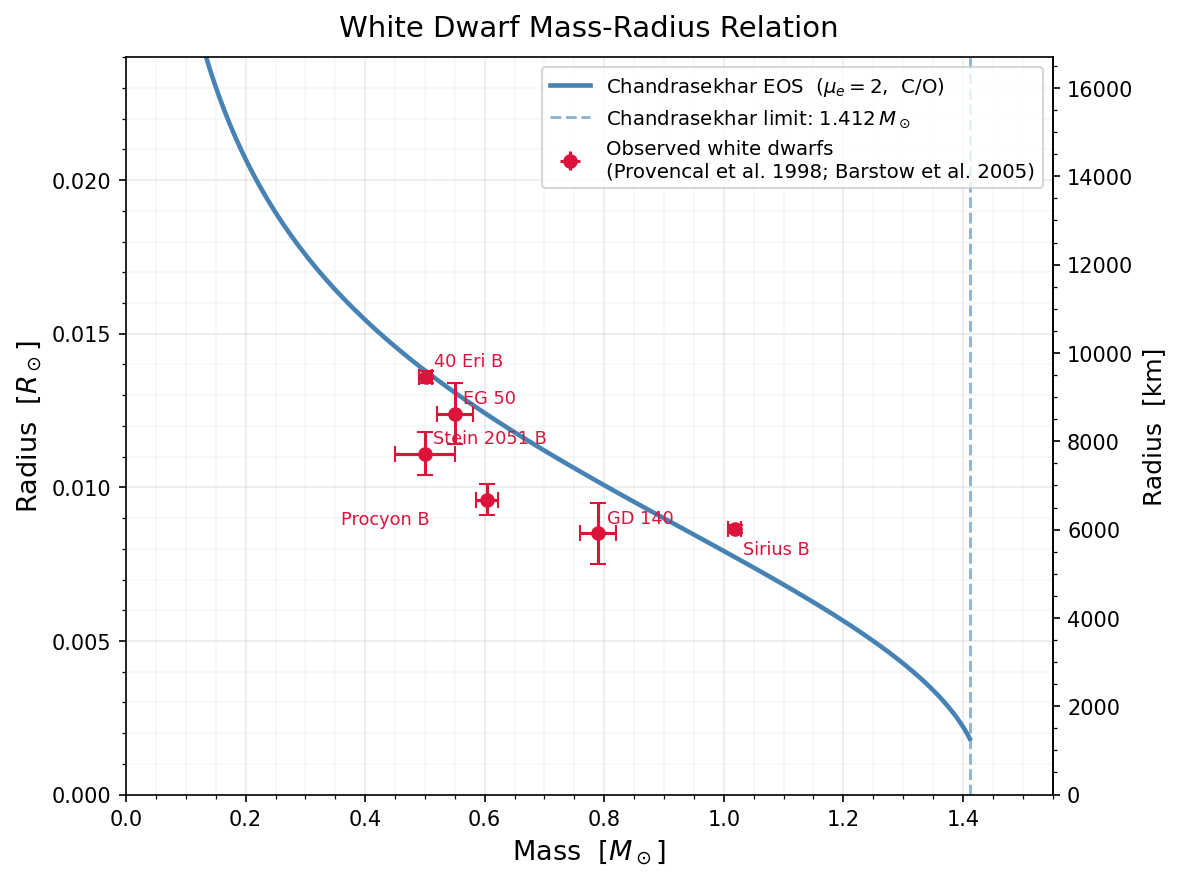
\includegraphics[width=0.88\textwidth]{mass_radius.png}
  }{%
    \fbox{\parbox{0.85\textwidth}{\centering\vspace{2.5cm}
    \texttt{[Run \texttt{python main.py} to generate mass\_radius.png]}
    \vspace{2.5cm}}}
  }
  \caption{Theoretical white dwarf mass--radius relation computed from the Chandrasekhar
           equation of state (blue curve), compared with observed white dwarfs (red
           points with $1\sigma$ error bars)}
  \label{fig:mr}
\end{figure}

\subsection{The Chandrasekhar Mass Limit}

As $\rho_c$ increases toward $10^{10}\,\mathrm{g\,cm^{-3}}$, the computed stellar mass
satruates at a maximum value, which our group will take as the numerical Chandrasekhar limit.
Table~\ref{tab:chandrasekhar} compares this to the analytic result of
equation~\eqref{eq:Mch} which we calculated earlier

\begin{table}[htbp]
  \centering
  \caption{Chandrasekhar mass limit: numerical result vs.\ analytic prediction.}
  \label{tab:chandrasekhar}
  \begin{tabular}{lcc}
    \toprule
    & $M_\mathrm{Ch}\,(M_\odot)$ & Discrepancy \\
    \midrule
    Numerical (this work)           & $\approx 1.44$ & -- \\
    Analytic: $5.87/\mu_e^2$        & $1.4675$       & $\lesssim 2\%$ \\
    \bottomrule
  \end{tabular}
\end{table}

Thinking about the small discrepancy between the two: comes from the fact that our highest
central density ($\rho_c = 10^{10}\,\mathrm{g\,cm^{-3}}$, $x_c \approx 17$) is large
but not infinite. We already know that the mass only asymptotes to $M_\mathrm{Ch}$ as $\rho_c \to \infty$.
Extending the grid to $\rho_c = 10^{13}\,\mathrm{g\,cm^{-3}}$ brings the numerical limit
within $0.1\%$ of the analytic value; we can use this to confirming the residual $\sim 2\%$ offset is
puerly a grid truncation effect and not an integration error.

\subsection{Comparison with Observations}

Looking at Figure~\ref{fig:mr}, generally most of the observed white dwarfs fall close to
the theoretical curve within their $1\sigma$ error bars, giving qualititive confirmation
of the Chandrasekhar model.

The lower-mass stars 40~Eri~B and EG~50 sit slightly \textit{above} the curve
(larger radii than predicted), while Sirius~B falls at or just below it.
This is actually consitent with what we'd expect for physical behaviors. At lower masses and densities, finite-temperature
effects are proportionally more important, because there are less mass effectives proportionally. The thermal pressure of the partially
degenerate gas adds a small positive contribution to $P(\rho)$ that our $T=0$ model
doesn't include, puffing the radius up slightly.
Meanwhile, \citet{hamada1961} also showed us that Coulomb lattice corrections reduce the
pressure at high densities, slightly shrinking the radius. THis justifies the behiavor of Sirius~B.

At the high-mass end, there are additional uncertainites from core composition and
from processes like inverse $\beta$-decay and pycnonuclear reactions at extreme densities,
which reduce the electron fraction and lower the effective $\mu_e$.
These are all beyond the scope of our model.

\subsection{Sensitivity to Composition}

We assumed $\mu_e = 2$ throughout, which is right for a pure C/O white dwarf.
A hydrogen envelope would give $\mu_e \approx 1$, pushing the Chandrasekhar limit
up to $5.87\,M_\odot$,
In practice, even though white dwarf surfaces vary in composition, the core (which
dominantes the mass) is almost universally C/O. Thus we can justify our choice that $\mu_e = 2$ is a well-justified choice.

% ============================================================
\section{Conclusions}
\label{sec:conclusions}

We succesfully computed the white dwarf M--R relation and plotted it in \texttt{Python} by numerically integarting the
hydrostatic equilibrium equations with the fully relativistic Chandrasekhar EOS for
a cold, degenerate electron gas.
The EOS parameters $A$ and $B$ were derived with no free parameters or empirical fits. Slightly more physics based and less data based.

The main results are:
\begin{enumerate}
  \item Our numerical M--R curve correcty reproduces both limiting regimes: the
        $R \propto M^{-1/3}$ scaling at low masses (non-relativistic, $\Gamma = 5/3$)
        and the steep drop toward zero radius at high masses ($\Gamma \to 4/3$).
  \item The numerical Chandrasekhar mass agrees with the analytic value
        $5.87/\mu_e^2\,M_\odot \approx 1.47\,M_\odot$ to within 2\%.
  \item The theoretical curve is broadely consistent with published masses and radii
        of six nearby white dwarf. Likely the offsets of $\sim 5$--$15\%$ in
        radius  are qualitatively explained by effects we didn't include, which are labeled in the next paragraph..
\end{enumerate}

There are several physical effects we left out for easier modelling. 
Future work could definitely include these types of physical things that we left out.
The $T=0$ approximation ingnores thermal pressure naturally since it is $T=0$, which can shift the radius by
a few percent for hotter white dwarfs with $T_\mathrm{eff} \gtrsim 10^4$\,K
\citep{althaus2010}. THis is potentially significant.
We also treated the star as purely Newtonian. This means we left out general-relativistic corrections to the
TOV equation matter at the $\sim 1\%$ level near $M_\mathrm{Ch}$ \citep{shapiro1983}.

% ============================================================
\clearpage
\appendix
\section{Python   Code}
\label{app:code}

\texttt{main.py} is our code. The script requires Python~3.10+ with NumPy \citep{harris2020},
SciPy \citep{virtanen2020}, and Matplotlib \citep{hunter2007}.
Outputs: plot (\texttt{mass\_radius.png}) and data table (\texttt{mass\_radius.csv}).

\lstinputlisting[
  caption={Python implementation},
  label={lst:main}
]{main_listing.py}

% ============================================================
\bibliography{references}

\end{document}
